% ==========================================
% REPORTE LATEX: PERSONA 3 - ANÁLISIS CINEMÁTICO
% Copia este código directamente en tu archivo de Overleaf (main.tex)
% ==========================================

\section{Representación Funcional y Parámetros Denavit-Hartenberg (DH)}

A partir del diseño del robot y el sistema de coordenadas establecido, se derivó la siguiente tabla de parámetros cinemáticos utilizando la convención estándar de Denavit-Hartenberg (DH):

\begin{table}[h!]
\centering
\begin{tabular}{|c|c|c|c|c|}
\hline
\textbf{Art. ($i$)} & \textbf{$\theta_i$ (Rotación $Z$)} & \textbf{$d_i$ (Offset $Z$)} & \textbf{$a_i$ (Longitud $X$)} & \textbf{$\alpha_i$ (Torsión $X$)} \\ \hline
\textbf{1 (Base)} & $q_1$ & $L_1 = 60.22\text{ mm}$ & $0$ & $-\pi / 2$ \\ \hline
\textbf{2 (Hombro)} & $q_2$ & $0$ & $L_2 = 459.72\text{ mm}$ & $0$ \\ \hline
\textbf{3 (Codo)} & $q_3$ & $0$ & $L_3 = 258.50\text{ mm}$ & $0$ \\ \hline
\textbf{4 (Muñeca)} & $q_4$ & $0$ & $L_4 = 28.00\text{ mm} + X_{\text{gripper}}$ & $0$ \\ \hline
\end{tabular}
\caption{Tabla de parámetros Denavit-Hartenberg (DH) del Brazo4.}
\label{tab:dh_parameters}
\end{table}

Donde $X_{\text{gripper}}$ representa la longitud añadida por el efector final de tijera acoplado ($\approx 60\text{ mm}$).

\subsection{Matrices de Transformación Homogénea}

Las matrices de transformación para cada articulación ($T_i$) que relacionan el eslabón $i$ con el $i-1$ son:

\begin{equation*}
T_1 = \begin{bmatrix} 
\cos q_1 & 0 & -\sin q_1 & 0 \\ 
\sin q_1 & 0 & \cos q_1 & 0 \\ 
0 & -1 & 0 & L_1 \\ 
0 & 0 & 0 & 1 
\end{bmatrix}
\quad
T_2 = \begin{bmatrix} 
\cos q_2 & -\sin q_2 & 0 & L_2 \cos q_2 \\ 
\sin q_2 & \cos q_2 & 0 & L_2 \sin q_2 \\ 
0 & 0 & 1 & 0 \\ 
0 & 0 & 0 & 1 
\end{bmatrix}
\end{equation*}

\begin{equation*}
T_3 = \begin{bmatrix} 
\cos q_3 & -\sin q_3 & 0 & L_3 \cos q_3 \\ 
\sin q_3 & \cos q_3 & 0 & L_3 \sin q_3 \\ 
0 & 0 & 1 & 0 \\ 
0 & 0 & 0 & 1 
\end{bmatrix}
\quad
T_4 = \begin{bmatrix} 
\cos q_4 & -\sin q_4 & 0 & L_4 \cos q_4 \\ 
\sin q_4 & \cos q_4 & 0 & L_4 \sin q_4 \\ 
0 & 0 & 1 & 0 \\ 
0 & 0 & 0 & 1 
\end{bmatrix}
\end{equation*}

\subsection{Cinemática Directa}

Multiplicando sucesivamente las matrices anteriores ($T_{total} = T_1 \cdot T_2 \cdot T_3 \cdot T_4$) y eliminando los componentes residuales numéricos del resolvedor, se obtiene la posición $[P_x, P_y, P_z]^T$ del efector final:

\begin{align*}
P_x &= \cos(q_1) \cdot \left[ L_4 \cos(q_2 + q_3 + q_4) + L_3 \cos(q_2 + q_3) + L_2 \cos(q_2) \right] \\
P_y &= \sin(q_1) \cdot \left[ L_4 \cos(q_2 + q_3 + q_4) + L_3 \cos(q_2 + q_3) + L_2 \cos(q_2) \right] \\
P_z &= L_1 - L_4 \sin(q_2 + q_3 + q_4) - L_3 \sin(q_2 + q_3) - L_2 \sin(q_2)
\end{align*}

\section{Análisis del Espacio de Trabajo (Workspace) y Manipulabilidad}

Se realizó una simulación numérica de Monte Carlo con $5000$ muestras aleatorias dentro de los límites articulares reales del robot: $q_1 \in [-\pi, \pi]$ y $q_2, q_3, q_4 \in [-\pi/2, \pi/2]$ rad.

\begin{figure}[h!]
\centering
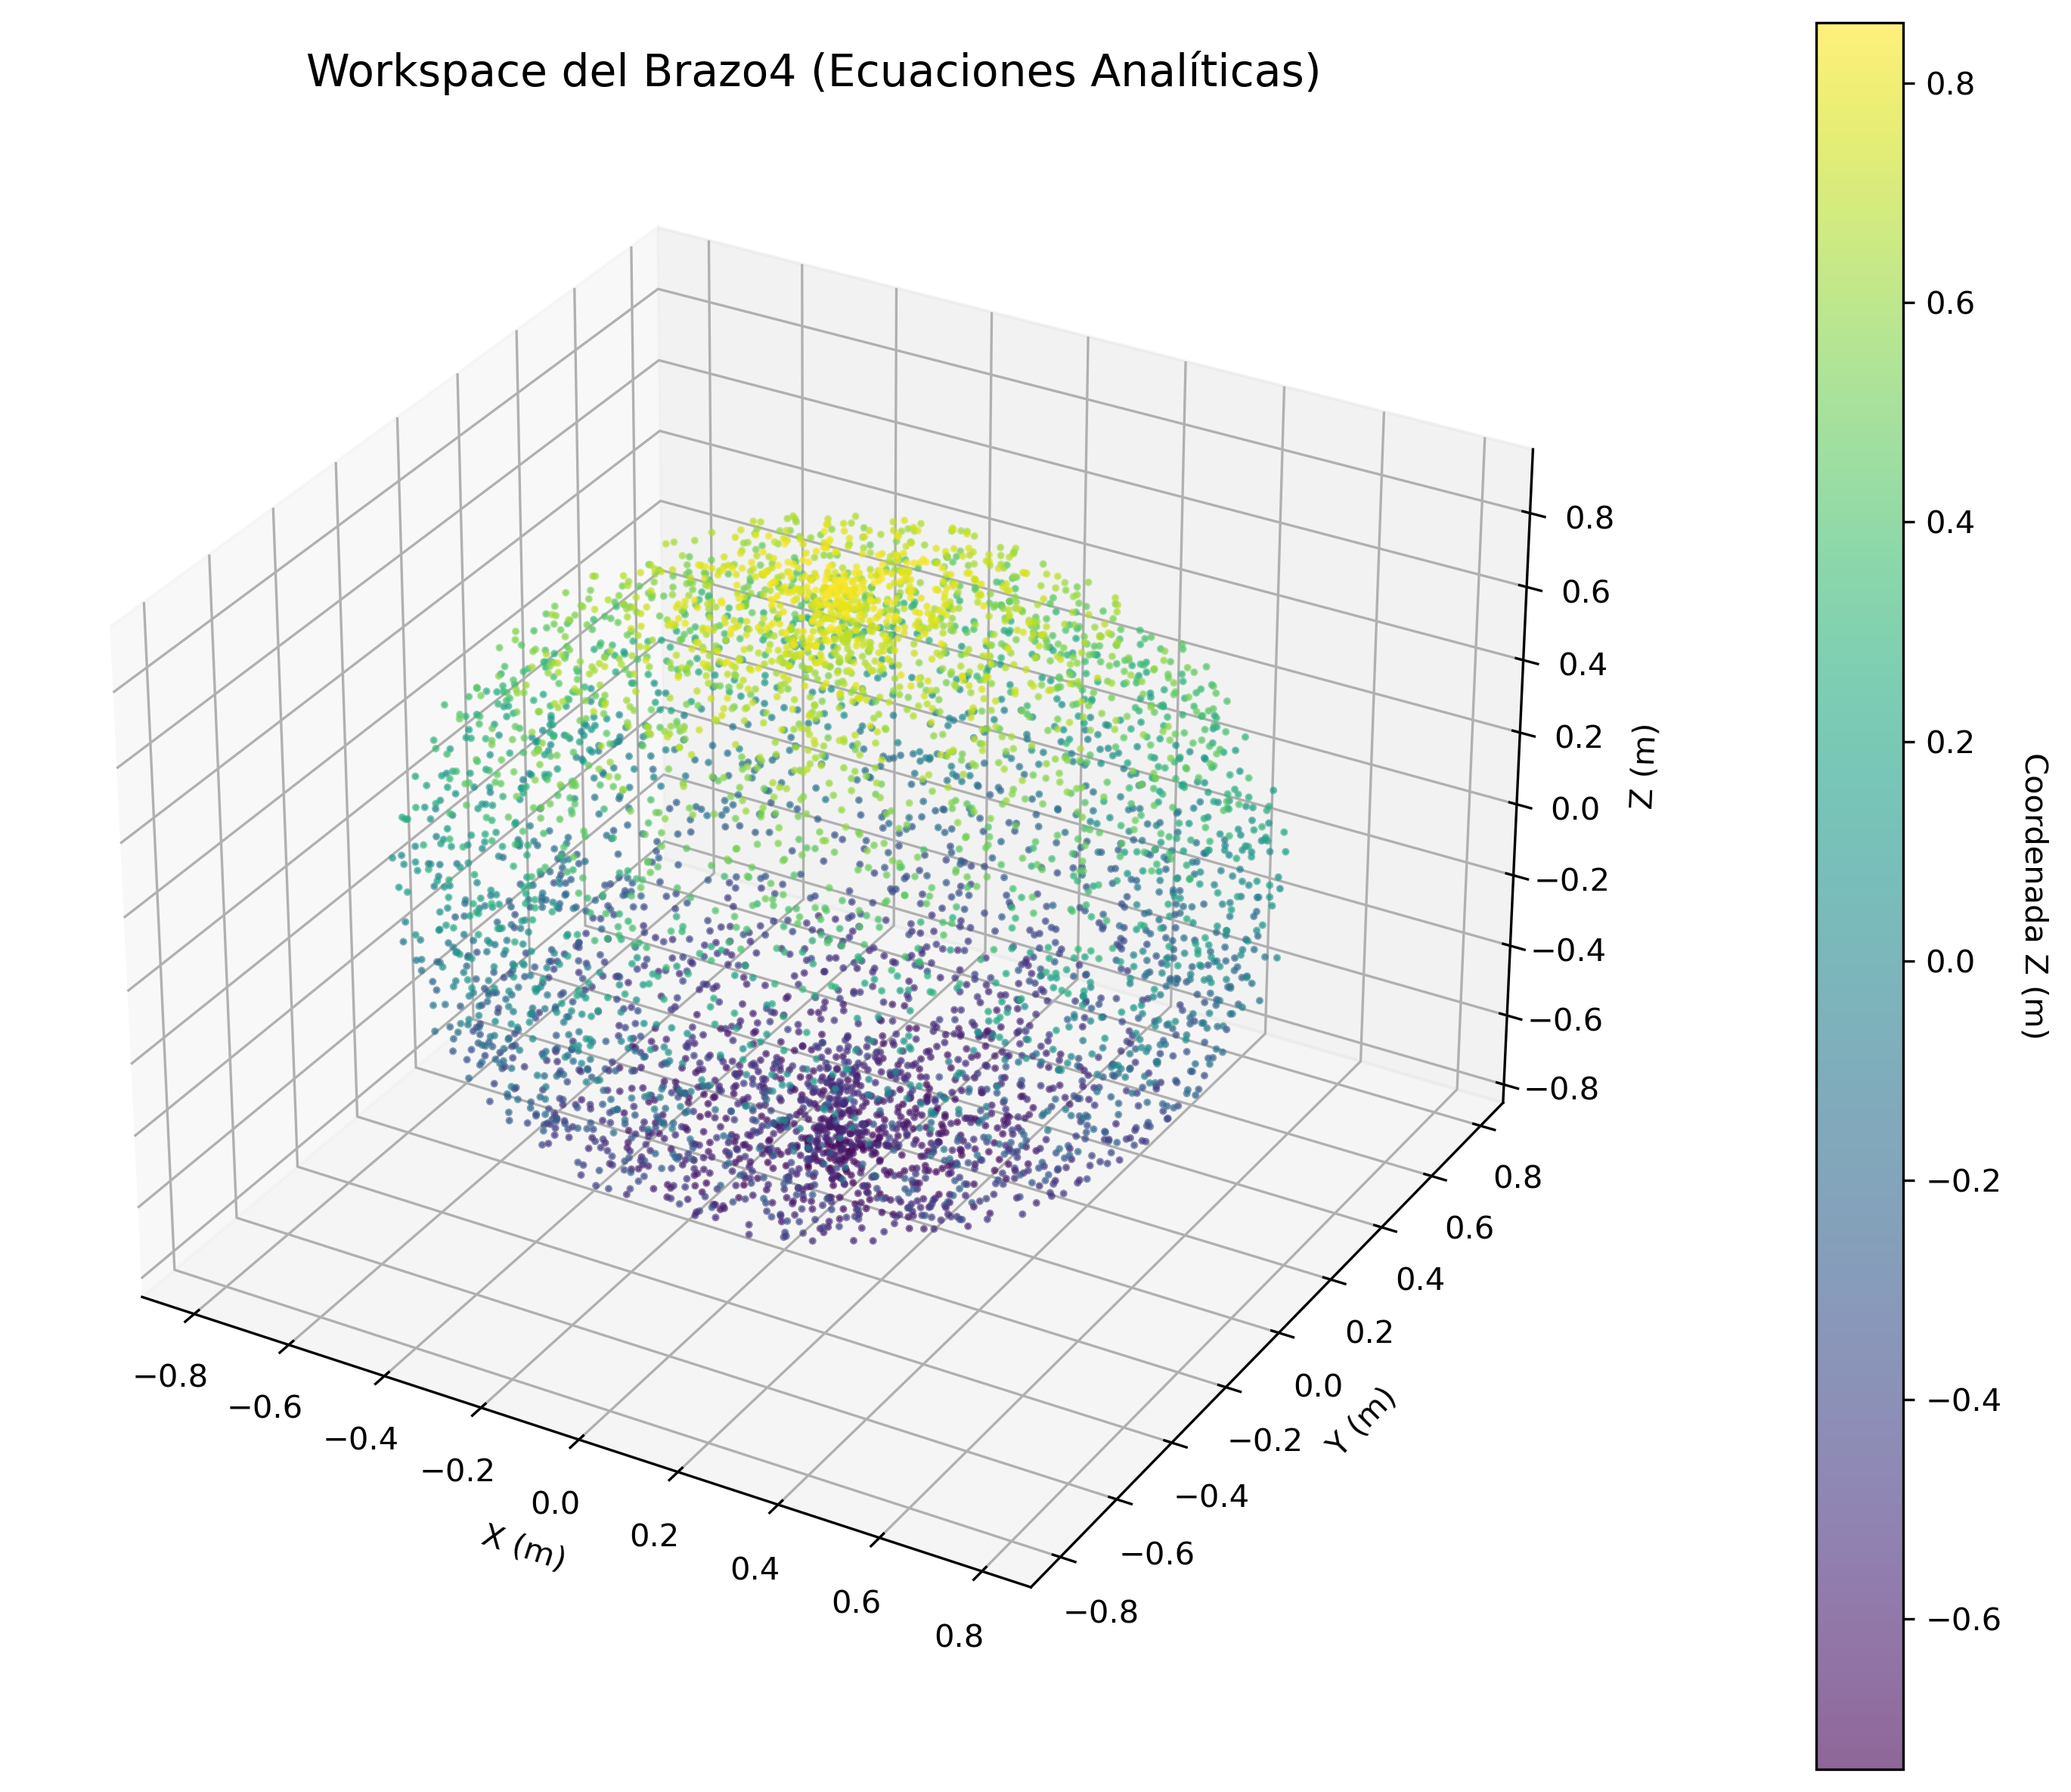
\includegraphics[width=0.75\textwidth]{workspace_brazo4.png}
\caption{Workspace 3D del Brazo4 mapeado con el índice de manipulabilidad de Yoshikawa.}
\label{fig:workspace}
\end{figure}

A partir de los resultados de la simulación, se extrajeron los siguientes límites físicos operacionales del manipulador:
\begin{itemize}
    \item \textbf{Alcance máximo radial:} $2.308\text{ m}$ (extensión máxima).
    \item \textbf{Alcance mínimo radial:} $0.889\text{ m}$ (zona de colisión propia).
    \item \textbf{Volumen de trabajo útil en Z:} $[0.724, 2.152]\text{ m}$ sobre el plano del suelo.
    \item \textbf{Manipulabilidad máxima ($w_{max}$):} $0.0670$ (Yoshikawa).
    \item \textbf{Manipulabilidad promedio ($w_{prom}$):} $0.0243$.
\end{itemize}

\section{Análisis de Singularidades}

El robot presenta tres tipos críticos de configuraciones singulares donde la destreza se anula:
\begin{enumerate}
    \item \textbf{Singularidad de frontera:} Ocurre con el brazo totalmente extendido ($q_3 = 0, q_4 = 0$). El robot pierde el grado de libertad radial.
    \item \textbf{Singularidad en el eje vertical central:} Ocurre cuando el efector se encuentra sobre el eje de rotación de la base ($P_x=0, P_y=0$). Movimientos infinitesimales requieren velocidades angulares infinitas en la base ($q_1$).
    \item \textbf{Singularidad de pliegue interno:} Ocurre cuando el brazo se retrae completamente sobre sí mismo ($q_3 = \pm \pi/2$ y $q_2 = \mp \pi/2$).
\end{enumerate}

\section{Propiedades Físicas e Inerciales}

\begin{table}[h!]
\centering
\begin{tabular}{|l|c|c|c|}
\hline
\textbf{Eslabón} & \textbf{Masa (kg)} & \textbf{Centro de Masa (xyz en m)} & \textbf{Inercias principales ($I_{xx}, I_{yy}, I_{zz}$)} \\ \hline
\textbf{BL} & 0.2166 & $[0.680, 0.025, 1.435]$ & $1.71 \times 10^{-4}, 2.74 \times 10^{-4}, 1.79 \times 10^{-4}$ \\ \hline
\textbf{L1} & 0.3920 & $[-0.000, -0.005, -0.076]$ & $1.03 \times 10^{-3}, 1.12 \times 10^{-3}, 3.75 \times 10^{-4}$ \\ \hline
\textbf{L2} & 0.6017 & $[-0.049, -0.003, -0.129]$ & $3.08 \times 10^{-3}, 2.61 \times 10^{-3}, 1.35 \times 10^{-3}$ \\ \hline
\textbf{L3} & 0.1502 & $[0.161, 0.022, -0.033]$ & $3.89 \times 10^{-5}, 2.23 \times 10^{-4}, 2.14 \times 10^{-4}$ \\ \hline
\textbf{L4} & 0.0310 & $[-0.002, -0.017, -0.004]$ & $9.25 \times 10^{-6}, 8.96 \times 10^{-6}, 8.83 \times 10^{-6}$ \\ \hline
\end{tabular}
\caption{Propiedades inerciales extraídas del modelo URDF en ROS.}
\label{tab:inerciales}
\end{table}
